%!TEX TS-program = lualatex
%!TEX encoding = UTF-8 Unicode

\documentclass[12pt, hidelinks]{exam}

\printanswers

\usepackage{graphicx}
	\graphicspath{{/Users/goby/Pictures/teach/163/lab/}
	{img/}} % set of paths to search for images

\usepackage{geometry}
\geometry{letterpaper, left=1.5in, bottom=1in}                   
%\geometry{landscape}                % Activate for for rotated page geometry
\usepackage[parfill]{parskip}    % Activate to begin paragraphs with an empty line rather than an indent
\usepackage{amssymb, amsmath}
\usepackage{mathtools}
	\everymath{\displaystyle}

\usepackage{fontspec}
\setmainfont[Ligatures={TeX}, BoldFont={* Bold}, ItalicFont={* Italic}, BoldItalicFont={* BoldItalic}, Numbers={Proportional, OldStyle}]{Linux Libertine O}
\setsansfont[Scale=MatchLowercase,Ligatures=TeX, Numbers={Proportional,OldStyle}]{Linux Biolinum O}
\setmonofont[Scale=MatchLowercase]{Linux Libertine Mono O}
\newfontfamily{\liningnum}[Numbers=Lining]{Linux Libertine O}
\usepackage{microtype}%

\usepackage[table]{xcolor}

\usepackage[bold-style=ISO]{unicode-math}
\setmathfont[Scale=MatchLowercase]{Tex Gyre Pagella Math}

\usepackage{tikz}

\usepackage{pifont} % Use the x mark in the final section.

\usepackage{booktabs}
\usepackage{multicol}


\usepackage{caption}
\captionsetup{format=plain, justification=raggedright, singlelinecheck=off,labelsep=period,skip=3pt} % Removes colon following figure / table number.

%\usepackage{caption}
%\captionsetup{font=small} 
%\captionsetup{singlelinecheck=false}
%\captionsetup[figure]{labelsep=period, format=plain}

\usepackage{longtable}
\usepackage{caption}
\captionsetup{format=plain, justification=raggedright, singlelinecheck=off,labelsep=period,skip=3pt} 

\usepackage{array}
\newcolumntype{L}[1]{>{\raggedright\let\newline\\\arraybackslash\hspace{0pt}}p{#1}}
\newcolumntype{C}[1]{>{\centering\let\newline\\\arraybackslash\hspace{0pt}}p{#1}}
\newcolumntype{R}[1]{>{\raggedleft\let\newline\\\arraybackslash\hspace{0pt}}p{#1}}

\usepackage{enumitem}
\setlist{leftmargin=*}
\setlist[1]{labelindent=\parindent}
\setlist[enumerate]{label=\textsc{\alph*}.}
\setlist[itemize]{label=\color{white}\textbullet}

\usepackage{hyperref}
%\usepackage{placeins} %PRovides \FloatBarrier to flush all floats before a certain point.
\usepackage{hanging}

\usepackage[sc]{titlesec}

%% Commands for Exam class
\renewcommand{\solutiontitle}{\noindent}
\unframedsolutions
\SolutionEmphasis{\bfseries}

\renewcommand{\questionshook}{%
	\setlength{\leftmargin}{-\leftskip}%
}

%Change \half command from 1/2 to .5
\renewcommand*\half{.5}

\pagestyle{headandfoot}
\firstpageheader{\textsc{bi}\,063 Evolution and Ecology}{}{\ifprintanswers\textbf{KEY}\else Name: \enspace \makebox[2.5in]{\hrulefill}\fi}
\runningheader{}{}{\footnotesize{pg. \thepage}}
\footer{}{}{}
\runningheadrule

\newcommand*\AnswerBox[2]{%
    \parbox[t][#1]{0.92\textwidth}{%
    \begin{solution}#2\end{solution}}
    \vspace{\stretch{1}}
}

\newenvironment{AnswerPage}[1]
    {\begin{minipage}[t][#1]{0.92\textwidth}%
    \begin{solution}}
    {\end{solution}\end{minipage}
    \vspace{\stretch{1}}}

\newlength{\basespace}
\setlength{\basespace}{5\baselineskip}


\newcommand\chisq{$\chi^2$}
\newcommand*\meanY{\overline{Y}\kern0.67pt}

\newcommand*\AnswerBlank[1]{%
	\ifprintanswers%
		\textbf{#1}
	\else%
		\rule{0.75in}{0.4pt}\kern0.67pt.\fi%
	}

%\newcommand*\AnswerBlank{\rule{0.75in}{0.4pt}\kern0.67pt.}
\newcommand*\xcell[1]{cell~\liningnum{#1}}

%
%\makeatletter
%\def\SetTotalwidth{\advance\linewidth by \@totalleftmargin
%\@totalleftmargin=0pt}
%\makeatother



\begin{document}

\subsection*{Resource partitioning: \textit{Bombus} bumble bees}

Resource partitioning allows more species to co-occur in a community.
Coexisting species that use one or more resources in the same way compete
with each other for the resources. Competition is reduced if species
use resources in different ways.

\textbf{Build but keep it short}


You will analyze several data sets to explore resource partitioning for five
species of bumble bees in the genus \textit{Bombus.} These data were collected
by Macior (1974), Pyke (1982), and Pyke et~al.~(2012) near Crested Butte, Colorado,
southwest of Denver. \textbf{Put map in pre-lab.}

Researchers walked transects (paths) counting species of bumble bees and the 
species of flowers visited by the bees for pollen and nectar. They walked
three transects and counted a total of 13,136 individuals for 12 species of 
\textit{Bombus} (Pyke 1982).

For simplicity, you'll use data for five of the species most commonly sighted along two of the transects.


\subsubsection*{Analysis: proboscis lengths}

Download bombus\_data.xlsx\footnote{All data currently in one
spreadsheet.} and click on the “Proboscis Lengths” tab. These data are
 proboscis lengths from 50 individuals for each of five \textit{Bombus} species. All measurements are in millimeters (mm).\footnote{Data simulated 
from results of Macior (1974).}

Use the \texttt{average} function in Excel to calculate the mean $\left(\meanY\right)$ proboscis length for each species. Use the \texttt{stdev.s} function
to calculate the sample standard deviation $\left(s\right)$ for each species. %Use the \texttt{count} and \texttt{sqrt} functions to calculate standard 
%error of the mean. As a reminder, the equation to calculate $\mathrm{SE}_{\meanY}$ is
%
%\begin{equation*} \label{eq:stderr}
%\mathrm{SE}_{\meanY} = \dfrac{s}{\sqrt{n}}
%\end{equation*}
%
%where $s$ is the standard deviation of the sample and $n$ is the sample size. 

\newpage

\begin{questions}

\question
Fill in the blanks with the mean $\left(\meanY\right)$ proboscis lengths and
sample standard deviation $\left(s\right)$ for the five \textit{Bombus} 
species. Round your results to one decimal place.

\begin{tabular}{@{}lcc@{}}
\toprule
Species & $\meanY$ & $s$ \tabularnewline
\midrule
& &  \tabularnewline
\textit{B.~appositus} & 
\ifprintanswers \textbf{12.8} \else \rule{1in}{0.4pt} \fi &
\ifprintanswers \textbf{0.4} \else \rule{1in}{0.4pt}  \fi 
\tabularnewline[2em]
%
\textit{B.~bifarius} &
\ifprintanswers \textbf{8.5} \else  \rule{1in}{0.4pt} \fi &
\ifprintanswers \textbf{0.4} \else \rule{1in}{0.4pt} \fi 
\tabularnewline[2em]
%
\textit{B.~frigidus} & 
\ifprintanswers \textbf{7.3} \else \rule{1in}{0.4pt} \fi &
\ifprintanswers \textbf{0.3} \else \rule{1in}{0.4pt} \fi 
\tabularnewline[2em]
%
\textit{B.~kirbiellus} &
\ifprintanswers \textbf{12.1} \else \rule{1in}{0.4pt} \fi & 
\ifprintanswers \textbf{0.4} \else \rule{1in}{0.4pt} \fi 
\tabularnewline[2em]
%
\textit{B.~sylvicola} & 
\ifprintanswers \textbf{8.4} \else \rule{1in}{0.4pt} \fi & 
\ifprintanswers \textbf{0.5} \else \rule{1in}{0.4pt} \fi 
\tabularnewline

\bottomrule
\end{tabular}

\bigskip

\question
Sketch a graph of the means with their standard deviations. Mark a 
large point above each species name at the proper height for the 
mean. Draw a thin vertical line that extends above and below the 
mean by the amount of the deviation. For example, if the mean is 
10.2~mm and the standard deviation is 0.4~mm, mark a point at 
10.2, and then draw a thin line from 9.8 (10.2\,$-$\,0.4) to
10.6 (10.2\,$+$\,0.4). 

\ifprintanswers
	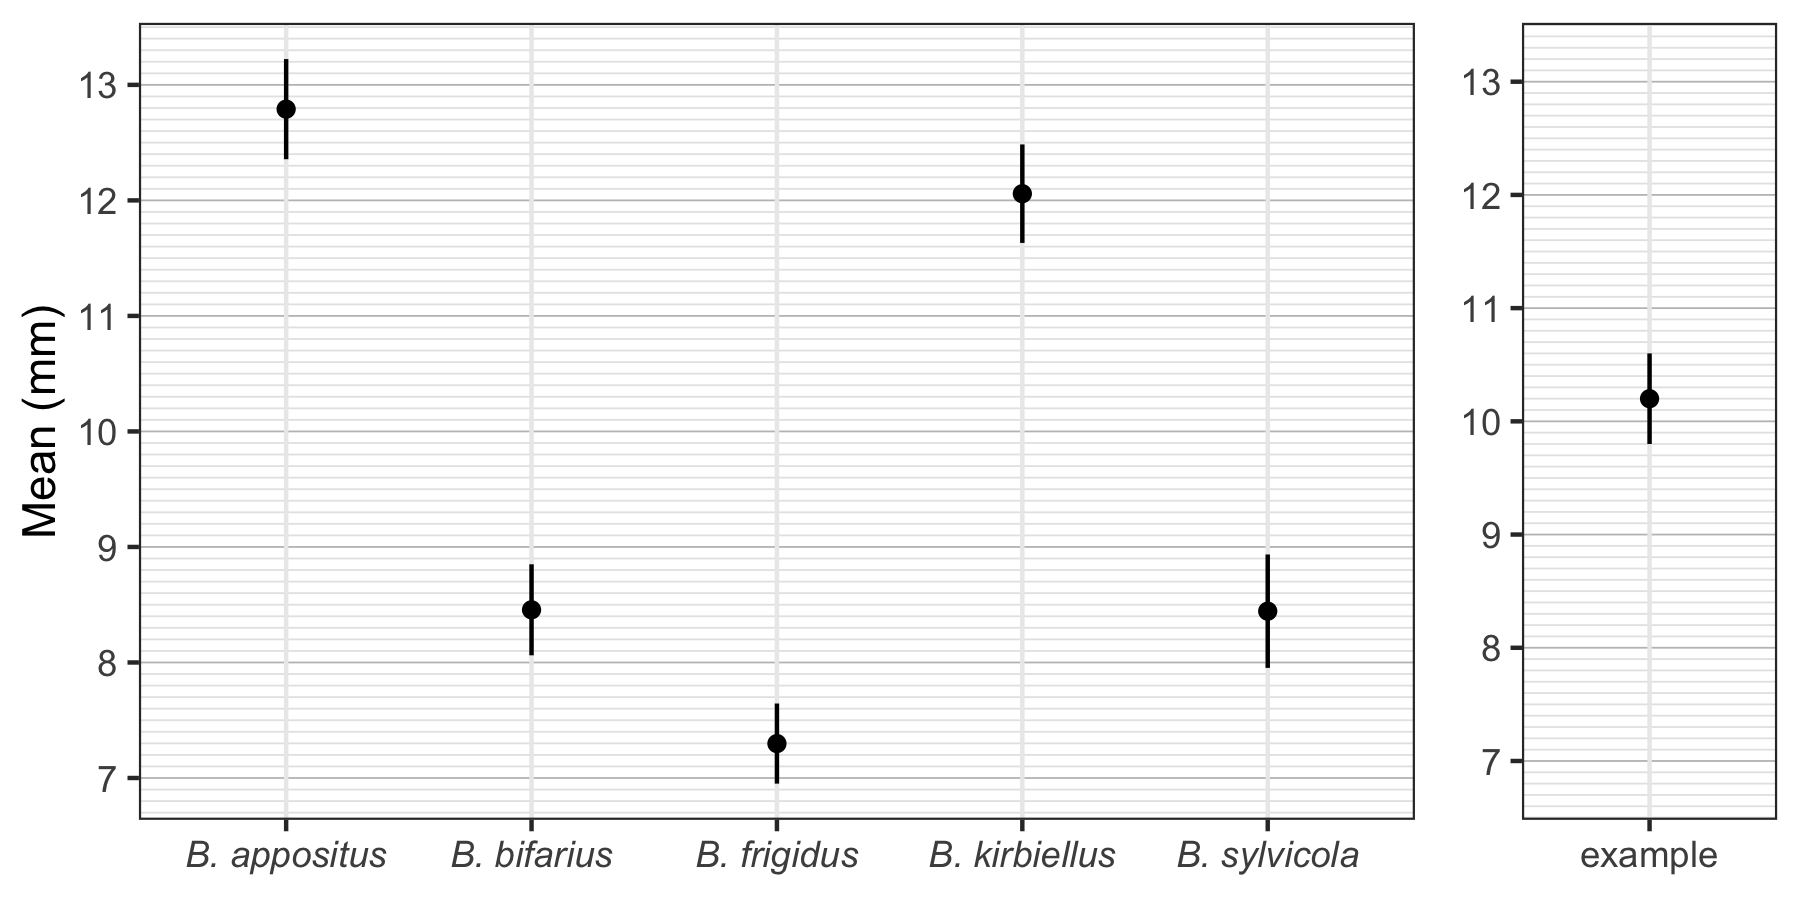
\includegraphics[width=\textwidth]{mean_proboscis_plot_key}
\else
	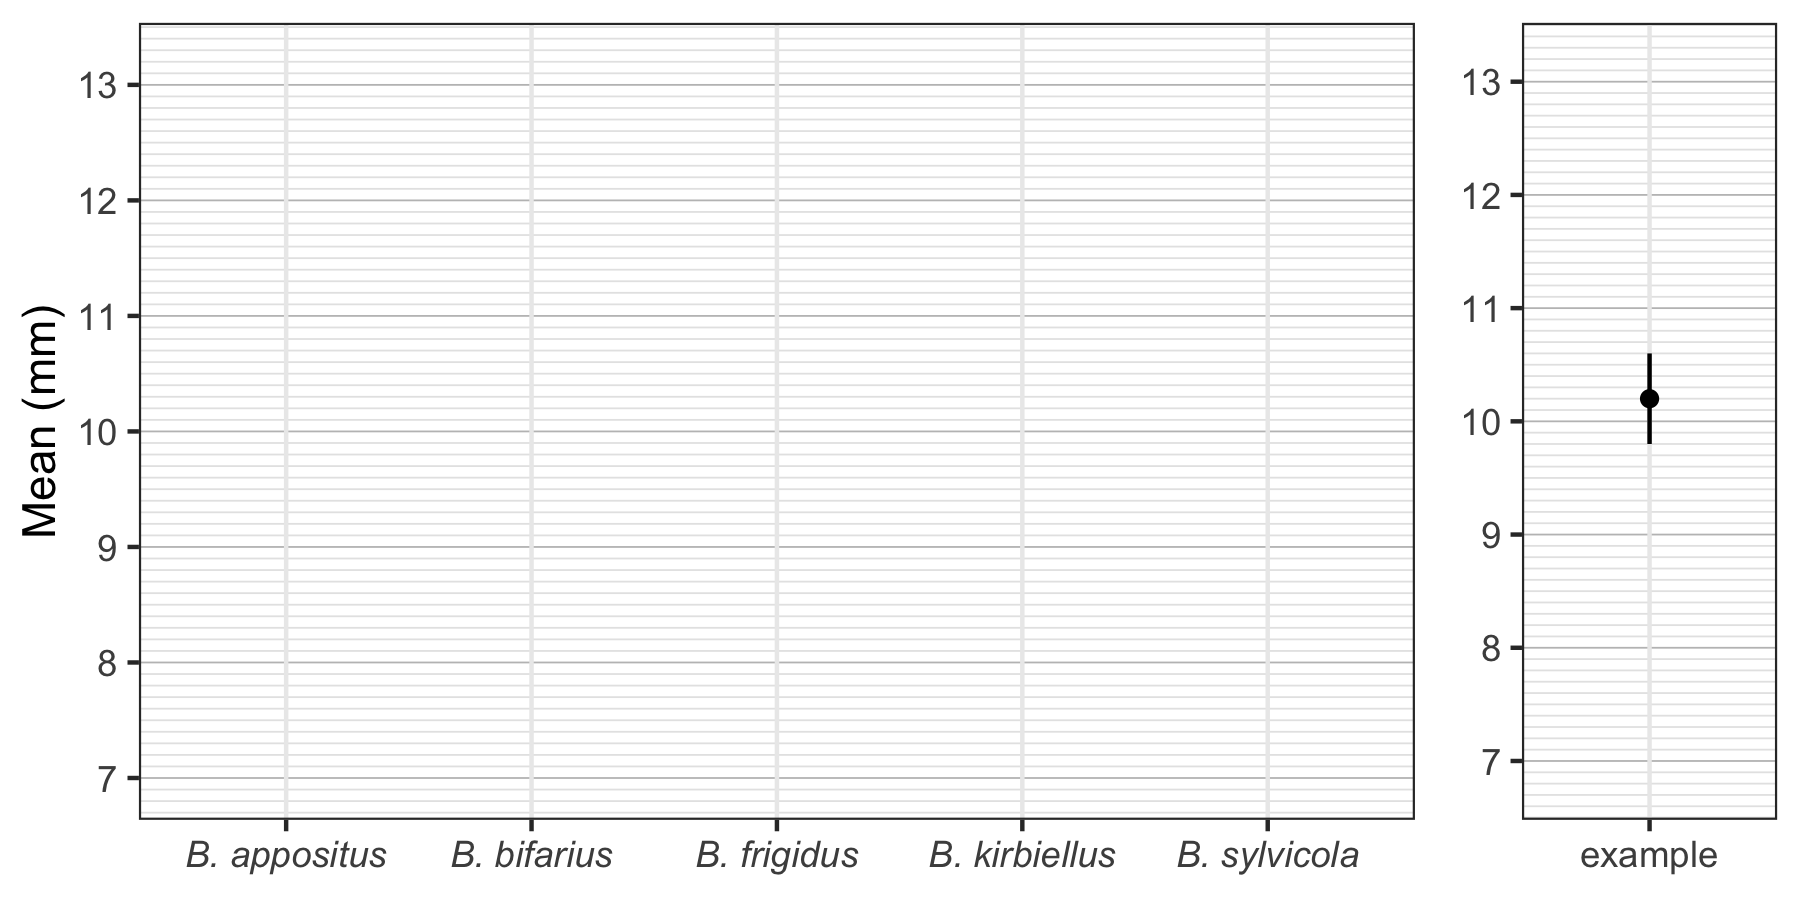
\includegraphics[width=\textwidth]{mean_proboscis_plot_blank}
\fi

\textbf{Consider adding student-built histogram plots, or a shiny 
	app for histograms to show spread and overlap of data.}

\question
The results suggest two size classes of \textit{Bombus}, based on
proboscis lengths.  Write the names of each species that belongs in 
each group.

\begin{tabular}{@{}ll@{}} %% ADD BLANKS for HANDOUTS.
	\toprule
	Short proboscis & Long proboscis \tabularnewline
	\midrule
	& \tabularnewline
	\ifprintanswers \textbf{\textit{B. bifarius}} \else \rule{2in}{0.4pt} \fi &
	\ifprintanswers \textbf{\textit{B. appositus}} \else \rule{2in}{0.4pt} \fi 
	\tabularnewline[2em]
	%
	\ifprintanswers \textbf{\textit{B. frigidus}} \else \rule{2in}{0.4pt} \fi &
	\ifprintanswers \textbf{\textit{B. kirbiellus}} \else \rule{2in}{0.4pt} \fi
	\tabularnewline[2em]
	%
	\ifprintanswers \textbf{\textit{B. sylvicola}} \else \rule{2in}{0.4pt} \fi &
	\rule{1in}{0.4pt} \tabularnewline
	\bottomrule
\end{tabular}

\textbf{Consider ANOVA to test for differences in proboscis lengths. 
	Shiny app?}

\bigskip

\question
Could proboscis length affect the flower size chosen by the bumble bees? Write a single sentence hypothesis that addresses this question. \textbf{Wording?}

\AnswerBox{2\baselineskip}{The length of the proboscis determines the size
	of the flowers chosen by bumble bees.}

\question
Write a prediction based on your hypothesis.

\AnswerBox{3\baselineskip}{If proboscis length determines flower size chosen, then \textit{Bombus} species with short proboscises will chose smaller flowers than species with longer proboscises.}


\subsubsection*{Analysis: proboscis length and corolla length}\label{sec:proboscis_flower_length}

\textbf{Inc. pic of flower corolla? Or put in pre-lab?}

Pyke et al.~(2012) measured the corolla lengths for all species of flowers visited by different species and castes (queens, workers, and males) of \textit{Bombus.} You will find the average corolla and proboscis lengths recorded in the “Proboscis and Corolla Lengths” tab. 

\question
Make a scatterplot of the data with proboscis length on the x-axis and corolla length on the y-axis.

\ifprintanswers
	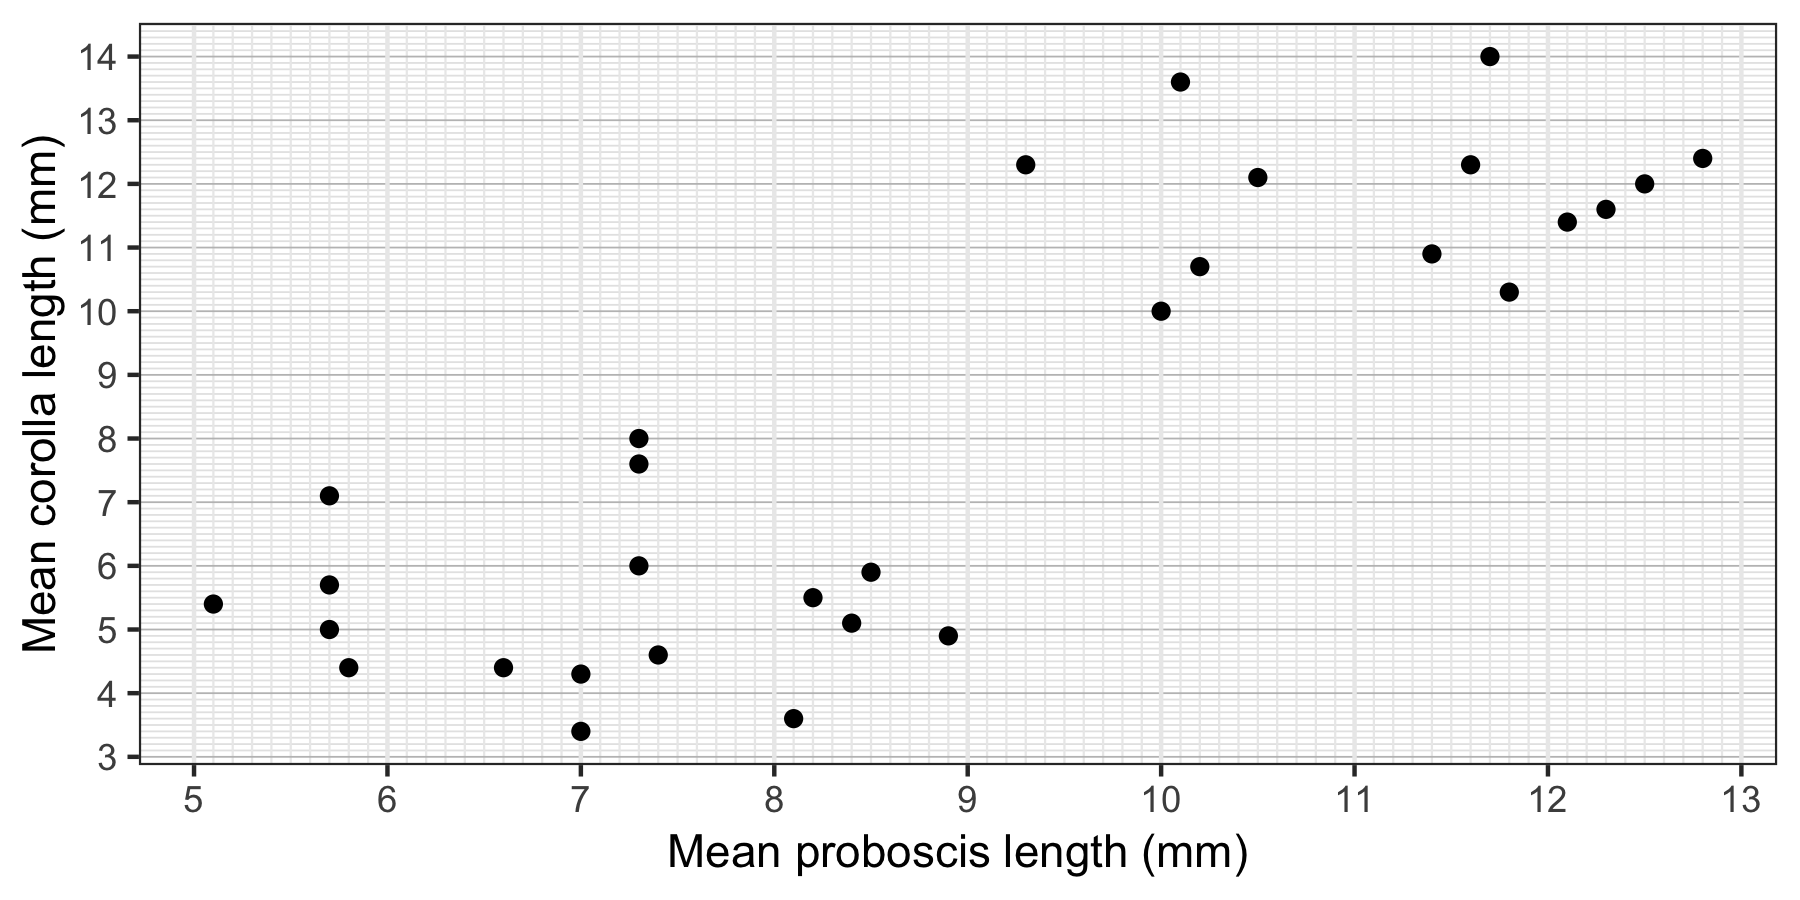
\includegraphics[width=\textwidth]{proboscis_corolla_key}
\else
	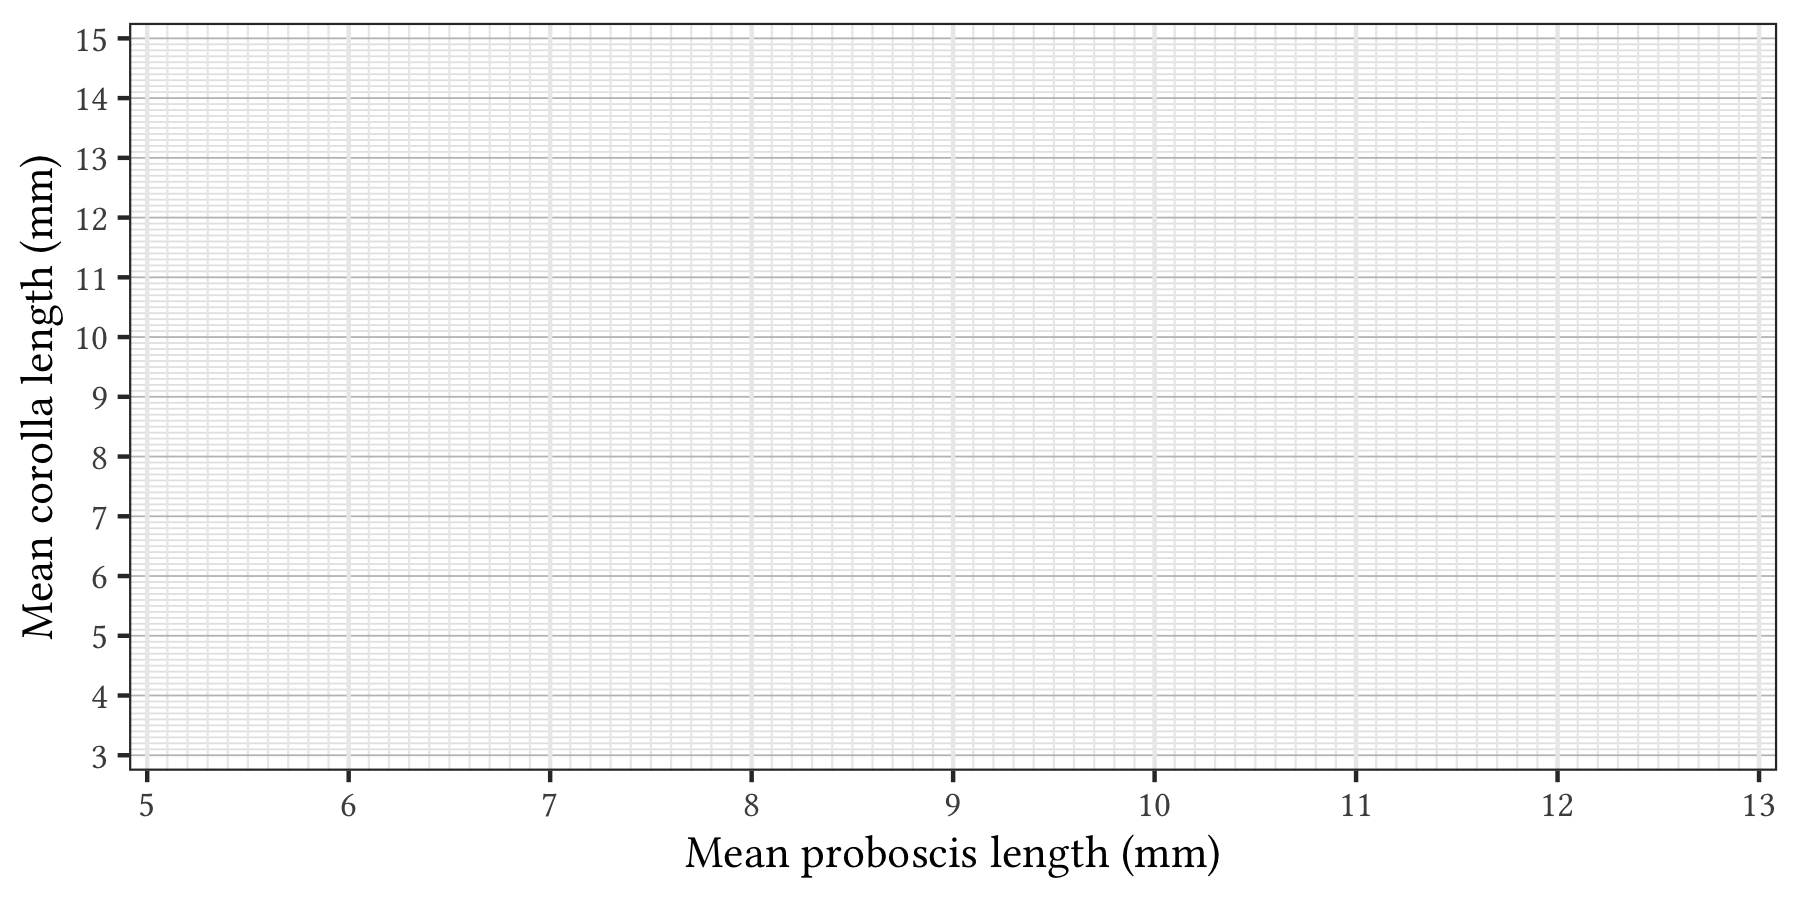
\includegraphics[width=\textwidth]{proboscis_corolla_blank}
\fi

\question
Do the results agree with your prediction? Explain.

\AnswerBox{3\baselineskip}{The scatterplot shows two clusters of points. 
\textit{Bombus} species with long proboscises tend to visit plant species with 
long corollas. \textit{Bombus} species with short proboscises tend to visit plant species with short corollas.}


\subsubsection*{Analysis: flower visitation by \textit{Bombus}}

The scatterplot you made was based on average values for proboscis and corolla 
lengths. Does this mean that \textit{Bombus} visited \emph{only} size-appropriate flowers?  

To answer this question Pyke (1982) recorded the flower species visited by the five \textit{Bombus} species. They recorded 7,161 visits to 34 plant species. Corolla lengths ranged from 0-27.2 mm. You will find their data in the “Flower visits” tab.

To graph the data, Pyke grouped the flowers into four classes based on corolla length.

0–3.99 mm\newline
4–7.99 mm\newline
8–11.99 mm\newline
12$+$ mm

\question
Tally the number of visits by each species of \textit{Bombus} to each size class of flowers. \textbf{Wording?}

\emph{Follow the following instructions carefully.}

\begin{enumerate}
	\item Enter 0 mm, 4 mm, 8 mm, and 12 mm into cell row J1 to M1 (one per cell)
	to represent the \emph{minimum} corolla length needed for each size class.
	
	\item Enter the five species names into column I2 to I6.
	
	\textsc{Calculate} the number of visits by \textit{B.~appositus} to the four
	size classes of flowers. 
	
	\item Click in cell J2, and then use the \textsc{sum} function to add the
	number of flower visits in the \textit{B. appositus} column with corolla
	lengths less than 3.99. For this cell, you should sum cells C28 to C35. 
	(You can sum only the cells with values, if you wish.)
	
	\item Click in cell K2. Sum the values for \textit{B. appositus} for
	all plant species with corolla lengths between 4–8.9 mm. 
	
	\item Click in cell L2 and sum the values for \textit{B. appositus} for
	all plant species with corolla lengths between 8–11.9 mm.
	
	\item Click in cell M2 and sum the values for \textit{B. appositus} for
	all plant species with corolla lengths 12 mm or longer.
	
	\item Repeat this process for the four remaining species. You can ask your instructor to check to be sure your results look correct. 
	
\end{enumerate}

\question
Use the values in your table to sketch separate bar charts for the number
of visits to each size class for each species of \textit{Bombus}.


\textbf{Anything about flower choice? That is more difficult to tease apart
	but would maybe work with guidance for select plant species.}


\subsubsection*{Interpretation: proboscis length and flower size.}

\question[Checkout]
Do the results so far provide evidence of resource partitioning?  Explain.

\AnswerBox{2\baselineskip}{So far, the results suggest that partitioning
occurs between species with short versus long proboscises. However, bumble
bees with similar proboscis lengths use similar size flowers.}

\subsubsection{Analysis: altitude and relative abundance}






\question[Checkout]
Describe the evidence you now have and how it supports resource partitioning among the five species of \textit{Bombus} bumble bees studied here.


\end{questions}


\subsubsection*{Literature Cited}

\begin{hangparas}{\leftmargin}{1}

Macior, L.\,W. 1974. Pollination ecology of the front
range of the Colorado Rocky Mountains. Melanderia 15: 1–59.

Pyke, G.\,H. 1982. Local geographic distributions of bumblebees 
near Crested Butte, Colorado: competition and community structure.
Ecology 63: 555–573.

Pyke, G.\,H., D.\,W.\,Inouye, and J.\,D.\,Thomson. 2012. Local geographic distributions of bumble bees near Crested Butte, Colorado: competition and community structure revisited. Environmental Entomology 41: 1332–1349.

\end{hangparas}

\end{document}  